\chapter{Hyperbolic Equations in Two Variables : Elliptic, Hyperbolic \&\ Parabolic Operators}

\setcounter{pageoriginal}{0}
Let\pageoriginale $\Omega$ be an open set in $\mathbb{R}^{2}$ and
$$
L=A\frac{\partial^{2}}{\partial x^{2}}+2B\frac{\partial^{2}}{\partial x\partial y}+C\frac{\partial^{2}}{\partial y^{2}}+D\frac{\partial}{\partial x}+E\frac{\partial}{\partial y}+G
$$
be a second order linear differential operator in $\Omega$ where $(A,B,\ldots,G)$ are smooth $(c^{\infty})$ functions in $\Omega$.

\begin{defi*}
Let $(x_{0},y_{0})\in \Omega$. We say that the operator $L$ is elliptic at $(x_{0},y_{0})$ if the characteristic form
$$
A(x_{0},y_{0})\xi^{2}_{1}+2B(x_{0},y_{0})\xi_{1}\xi_{2}+C(x_{0},y_{0})\xi^{2}_{2}
$$
is definite i.e. if $(B^{2}-AC)(x_{0},y_{0})<0$. $L$ is said to be hyperbolic at $(x_{0},y_{0})$ if the characteristic form is indefinite i.e. $(B^{2}-AC)(x_{0},y_{0})>0$.
\end{defi*}

$L$ is said to be elliptic (resp. hyperbolic) in $\Omega$ if it is elliptic (resp. hyperbolic) at all points of $\Omega$. We shall define (provisionally) $L$ to be parabolic if the characteristic quadratic form is of rank 1 at every point.

\section*{The Wave Operator in Two Dimensions:}

We consider the wave operator $\dfrac{\partial^{2}}{\partial t^{2}}-\dfrac{\partial^{2}}{\partial x^{2}}$. The characteristic form is $\xi^{2}_{2}-\xi^{2}_{1}$. So this is an hyperbolic operator.

Make the change of variables $\xi=x+t$, $\eta=x-t$. We then have
$$
\frac{\partial}{\partial x}=\frac{\partial}{\partial \xi}+\frac{\partial}{\partial \eta}\quad\text{and}\quad \frac{\partial}{\partial t}=\frac{\partial}{\partial \xi}-\frac{\partial}{\partial\eta}\quad\text{so that}
$$
the wave operator goes over into the operator $4\dfrac{\partial^{2}}{\partial \xi \partial \eta}$.

Let\pageoriginale us consider the operator $\dfrac{\partial^{2}}{\partial \xi \partial \eta}$. The characteristic form is $\xi_{1}\xi_{2}$. A curve $C$ defined by $\phi=0$ with $d\phi\neq 0$ on $C$ will be characteristic if $\dfrac{\partial \phi}{\partial \xi}\cdot \dfrac{\partial \phi}{\partial \eta}=0$. We see that the curves $\xi$ = constant and $\eta$ = const. are characteristic curves.

If we look at the Cauchy problem $\dfrac{\partial^{2}u}{\partial\xi\partial\eta}=0$ and
$$
u(\xi,0)=\phi_{0}(\xi), \ \dfrac{\partial u}{\partial ???}(\xi,0)=\phi_{1}(\xi)\quad\text{on}\quad \eta=0,
$$
we see from
$$
\dfrac{\partial^{2}u}{\partial \xi \partial \eta}=0, \ \dfrac{\partial}{\partial \xi}\left(\dfrac{\partial u}{\partial \eta}\right)=0
$$
that $\phi_{1}(\xi)$ is constant. The curve $\eta=0$ is characteristic and we see that the Cauchy data cannot be prescribed arbitrarily; some compatibility conditions have to be satisfied. Even if we take $\phi_{1}(\xi)$ to be a const. say $C$, the solution is not unique: take $u(\xi,\eta)=\phi_{0}(\xi)+f(\eta)$ where $t$ is any function with $f'(0)=C$ and $f(0)=0$.

From $\dfrac{\partial^{2}u}{\partial \xi\partial\eta}=0$ we have $\dfrac{\partial}{\partial\eta}\left(\dfrac{\partial u}{\partial\xi}\right)=0$ so that
$$
\frac{\partial u(\xi,\eta)}{\partial \xi}=f(\xi)
$$
so that $u(\xi,\eta)=\int f(\xi)d\xi+G(\eta)$, $G(\eta)$ being the constant of integration. Thus $u=F(\xi)+G(\eta)$; if $F(\xi)$ and $G(\xi)$ are smooth functions, it is clear that $F(\xi)+G(\eta)$ is a solution. Going back to the original variables, we see that
$$
u(x,t)=F(x+t)+G(x-t)
$$
is a solution of the wave operator.

We seek the solution of the Cauchy problem for the wave operator with initial data $u(x,0)=f(x)$; $\dfrac{\partial u}{\partial t}(x,0)=g(x)$, in the form $u=F(x+t)+G(x-t)$. We must have 
$$
u(x,0)=F(x)+G(x)=f(x)
$$\pageoriginale
and
$$
\frac{\partial u}{\partial t}(x,0)=F'(x)-G'(x)=g(x).
$$
Differentiating the first equation, we have $F'(x)+G'(x)=f'(x)$.

\smallskip

Thus $F'(x)=\dfrac{f'(x)+g(x)}{2}$  \ and \ $G'(x)=\dfrac{f'(x)-g(x)}{2}$ \ or
\begin{align*}
F(x) &= \dfrac{f(x)}{2}+\dfrac{1}{2}\int\limits^{x}_{0}g(\xi)d\xi+C_{1}\\[3pt]
G(x) &= \dfrac{f(x)}{2}-\dfrac{1}{2}\int\limits^{x}_{0}g(\xi)d\xi+C_{2}
\end{align*}

From $u(x,0)=f(x)$ we see that $C_{1}+C_{2}=0$. Hence
$$
u(x,t)=\dfrac{1}{2}\{f(x+t)+f(x-t)\}+\frac{1}{2}\int\limits^{x+t}_{x-t}g(\xi)d\xi.
$$

\begin{theorem*}
If $f$ is $C^{2}$ function and $g$ a $C^{1}$ function on $\mathbb{R}$, then the function $u(x,t)$ defined by
$$
u(x,t)=\dfrac{f(x+t)+f(x-t)}{2}+\dfrac{1}{2}\int\limits^{x+t}_{x-t}g(\xi)d\xi
$$
is a $C^{2}$ function in $t\geq 0$ and solves the Cauchy problem
$$
\begin{cases}
\dfrac{\partial^{2}u}{\partial t^{2}}-\dfrac{\partial^{2}u}{\partial x^{2}}=0\quad\text{in}\quad t\geq 0\\[5pt]
u(x,0)=f(x)\\[3pt]
\dfrac{\partial u}{\partial t}(x,0)=g(x).
\end{cases}
$$
\end{theorem*}

\begin{proof}
{\bf Exercise:}

The above solution of the Cauchy problem is called d'Alembert's solution.

Note the value of $u$ at $(x_{0},t_{0})$ depends only on the values of $f$ and $g$ on the closed interval $(x_{0}-t_{0}, x_{0}+t_{0})$ on the $x$-axis. These are the points\pageoriginale cut out on the axis by the characteristics $x-t=(x_{0}-t_{0})$ (= const.) and $x+t=(x_{0}+t_{0})$ passing through $(x_{0},t_{0})$. For this reason, the interval $(x_{0},-t_{0},x_{0}+t_{0})$ is called the interval or domain of dependence of the point $(x_{0},y_{0})$ (with respect to the wave operator).
\begin{figure}[H]
\centering
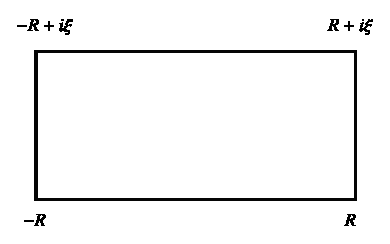
\includegraphics{1.eps}
\end{figure}

Conversely the initial values at a point $(\xi,0)$ on the $x$ - axis influence $u(x,t)$ only at points $(x,t)$ in the region bounded by the
\begin{figure}[H]
\centering
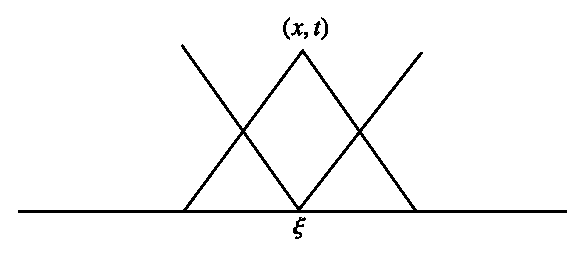
\includegraphics{2.eps}
\end{figure}
\noindent
characteristics $x+t=\xi$, $x-t=\xi$ i.e. in the region $\xi-t\leq x\leq \xi+t$. For this reason this region is called the domain of influence of the point $(\xi,\phi)$ on the $x$-axis.
\end{proof}

\begin{exer*}
Suppose that $f$ and $g$ have compact supports. Show that for each fixed $t$, the function $x\to u(x,t)$ has compact support.
\end{exer*}

Since any solution of $\dfrac{\partial^{2}u}{\partial t^{2}}-\dfrac{\partial^{2}u}{\partial x^{2}}=0$ is of the form $F(x+t)+G(x-t)$ the solution to the Cauchy problem is unique and is given by d'Alembert's formula.

\begin{exer*}
Let\pageoriginale $\{f_{n}\}$ (resp. $\{g_{n}\}$) be a sequence of $C^{2}$ (resp. $C^{1}$) functions which converges uniformly on compact subsets of $\mathbb{R}$ to a $C^{2}$ function $f$ (resp. $C^{1}$ function $g$). Show that the d'Alembert solution $u_{(f_{n},g_{n})}$ corresponding to the Cauchy data $(f_{n},g_{n})$ converges to the d'Alembert solution $u_{(f,g)}$ uniformly compact subsets of the upper half plane $t>0$.
\end{exer*}

Thus the Cauchy problem for the wave operator is well-posed.

\section{Cauchy Problem for the Nonhomogeneous Wave Equation:}

We consider the Cauchy problem
\begin{gather*}
\frac{\partial^{2}u}{\partial t^{2}}-\frac{\partial^{2}u}{\partial x^{2}}=F(x,t)\quad\text{it}\quad t\geq 0;\quad u(0,x)=f(x),\\[4pt]
\frac{\partial u}{\partial t}(0,x)=g(x),
\end{gather*}
where $F$, $f$ and $g$ are given. We will derive an explicit formula for the solution by applying Green's formula.

Let $\Omega$ be a bounded domain with piecewise smooth boundary. Let $u$ be a real valued function on $\Omega$. We shall say that $u$ is of class $C^{k}$ in $\overline{\Omega}$ if $u$ is of class $C^{k}$ in $\Omega$ and if $u$ and all partial derivatives of order upto $k$ admit continuous extensions to $\overline{\Omega}$. We shall denote the extended functions also by the original symbol.

\begin{exer*}
Let $\Omega$ be the interior of the rectangle (OABC).
\begin{figure}[H]
\centering
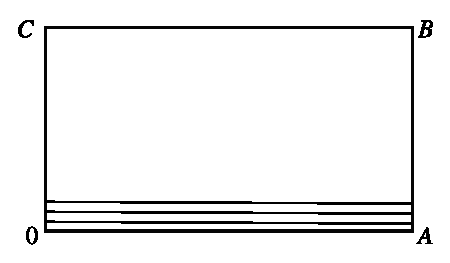
\includegraphics{3.eps}
\end{figure}
\noindent
where\pageoriginale $0A$ and $0B$ are the $x$ and $y$ axis. Let $f$ be a $C^{1}$ function on $\Omega$. Let $g(x)=f(x,0)$. Show that $g(x)$ is a $C^{1}$ function in the open interval $(0,A)$. Hint: (Consider a sequence of lines parallel to the $x$-axis and contained in the rectangle converging to $0A$).
\end{exer*}

We recall

\medskip
\noindent
{\bf Green's Formula:}~ Let $P$ and $Q$ be sufficiently smooth functions in $\overline{\Omega}$ where $\Omega$ is a bounded domain in $\mathbb{R}^{2}$ with a piecewise smooth boundary $\partial \Omega$. Then we have
$$
\iint_{\Omega}\left(\frac{\partial Q}{\partial x}-\frac{\partial p}{\partial y}\right)dx \ dy =\int\limits_{\partial \Omega}\ Pdx +Qdy.
$$
(The boundary is oriented ``anti-clockwise'')

\begin{coro*}
If $u$ is smooth, we have
$$
\iint\limits_{\Omega}\left(\frac{\partial^{2}u}{\partial t^{2}}-\frac{\partial^{2}u}{\partial x^{2}}\right)dx \ dt = \int\limits_{\partial\Omega}-\frac{\partial u}{\partial t}dx-\frac{\partial u}{\partial x}dt
$$

Apply this formula to the triangular region bounded by the characteristics $x-t=x_{0}-t_{0}$, $x+t=x_{0}+t_{0}$ and the $x$ - axis, where
\begin{figure}[H]
\centering
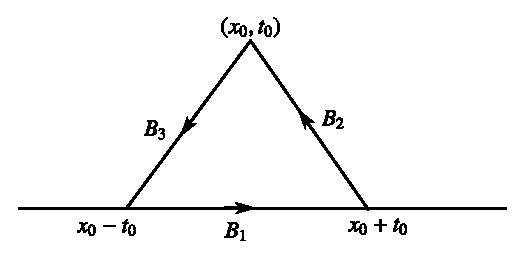
\includegraphics{4.eps}
\end{figure}
\noindent
$(x_{0},t_{0})$ is a point with $t_{0}>0$. If $u$ satisfies $\dfrac{\partial^{2}u}{\partial t^{2}}-\dfrac{\partial^{2}u}{\partial x^{2}}=F$, we have
$$
\int\limits_{B_{1}+B_{2}+B_{3}}-\frac{\partial u}{\partial t}dx-\dfrac{\partial u}{\partial x}dt=\int\limits_{\partial \Omega}-\frac{\partial u}{\partial t}dx-\dfrac{\partial u}{\partial x}dt=\int\limits_{\Delta} F\,dx\,dy
$$
where\pageoriginale $\Delta$ is in the interior of the triangle with vertices $(x_{0}-t_{0},0)$, $(x_{0}+t_{0},0)$, $(x_{0},t_{0})$ and $B_{1}$, $B_{2}$, $B_{2}$ are the sides of the triangle as indicated in the figure with their orientations.
\begin{enumerate}
\renewcommand{\labelenumi}{\rm(\theenumi)}
\item $\int\limits_{B_{1}}-\dfrac{\partial u}{\partial t}dx-\dfrac{\partial u}{\partial x}dt=-\int\limits^{x_{0}+t_{0}}_{x_{0}-t_{0}}\dfrac{\partial u}{\partial t}dx$

\item To evaluate the integral over $B_{2}$ consider the ``parametrisation'' $\phi(s)=(-s,s+x_{0}+t_{0})$ for $s$ in the closed interval $(-x_{0}-t_{0},-x_{0})$. We have $\phi(-x_{0}-t_{0})=(x_{0}+t_{0},0)$ and $\phi(x_{0})=(x_{0},t_{0})$. Since $dx=-dx$, $dt=ds$, and $\dfrac{d}{ds}=-\dfrac{\partial}{\partial x}+\dfrac{\partial}{\partial t}$
\begin{align*}
\int\limits_{B_{2}} \left(-\dfrac{\partial u}{\partial t}dx-\dfrac{\partial u}{\partial x}dt\right) &= \int\limits^{-x_{0}}_{-x_{0}-t_{0}}\left(\frac{\partial u}{\partial t}-\frac{\partial u}{\partial x}\right)ds\\[4pt]
&= \int\limits^{-x_{0}}_{-x_{0}-t_{0}}\left(\frac{du}{ds}\right)ds\\[4pt]
&= u(x_{0},t_{0}), u(x_{0}+t_{0},0)
\end{align*}

\item Consider the parametrisation of $B_{3}$ given by
$$
\psi(s)=(-s,-s-(x_{0}-t_{0}))
$$
for $s$ in the interval
$$
(-x_{0},-x_{0}+t_{0})\quad\text{with}\quad \psi(-x_{0})=(x_{0},t_{0}), \ \psi(-x_{0}+t_{0})=(x_{0}-t_{0},0).
$$

We have, as before
\begin{align*}
\int\limits_{B_{3}}\left(-\frac{\partial u}{\partial t}dx-\frac{\partial u}{\partial x}dt\right) &= \int\limits^{-x_{0}+t_{0}}_{-x_{0}}\left(\frac{\partial u}{\partial t}+\frac{\partial u}{\partial x}\right)ds\\[4pt]
&= -\int\limits^{-x_{0}+t_{0}}_{-x_{0}}\left(\frac{du}{ds}\right)ds\\[4pt]
&= u(x_{0},t_{0})-u(x_{0}-t_{0},0)
\end{align*}
\end{enumerate}

From\pageoriginale
$$
\int\limits_{B_{1}+B_{2}+B_{3}}=\int\limits_{\Delta}F \ dx \ dy,
$$
we get, from (1), (2) and (3) that
$$
u(x_{0},t_{0})=\frac{1}{2}\left\{u(x_{0}-t_{0},0)+u(x_{0}+t_{0},0)+\int\limits^{x_{0}+t_{0}}_{x_{0}-t_{0}}\left.\frac{\partial u}{\partial t}\right|_{t=0}dx+\int\limits_{\Delta} F \ dx \ dy\right\}
$$
\end{coro*}

\section*{Formula for the Solution of the Cauchy Problem:}\pageoriginale

What we have done above can be generalised a bit.
\begin{figure}[H]
\centering
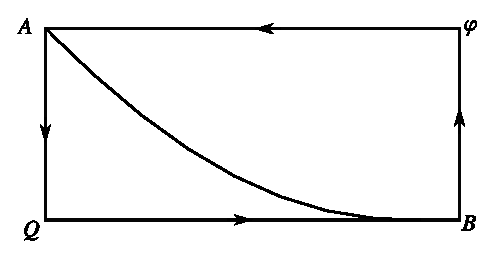
\includegraphics{5.eps}
\end{figure}

Let $S$ be a non-characteristic curve for the equation $\dfrac{\partial^{2}}{\partial x \partial y}$ i.e., $S$ is nowhere tangential to the lines $x$ = const. or $y$ = const. (More precisely the curve is given by $y=\sigma(x)$ with $\sigma'(x)<0$). Let $u$ be a solution of $\dfrac{\partial^{2}u}{\partial x\partial y}=F$ in the closed region $\overline{\Omega}$ bounded by $ABP$. We have by Green's formula
$$
\int\limits_{\Omega}\frac{\partial^{2}u}{\partial x\partial y}dx \ dy =\int\limits_{\partial\Omega}\frac{\partial u}{\partial y}dy=-\int\limits_{\partial \Omega}\frac{\partial u}{\partial x}dx
$$
Write these in the symmetrical form:
$$
\int\limits_{\Omega}\frac{\partial^{2}u}{\partial x\partial y}dx \ dy =\frac{1}{2}\int\limits_{\partial \Omega}\left(-\frac{\partial u}{\partial x}dx+\frac{\partial u}{\partial y}dy\right).
$$
Now
$$
\int\limits^{P}_{B}\left(-\frac{\partial u}{\partial x}dx+\frac{\partial u}{\partial y}dy\right)=\int\limits^{P}_{B}\frac{\partial u}{\partial y}dy=u(P_{0})-u(B)
$$
and
$$
\int\limits^{A}_{P}\left(-\frac{\partial u}{\partial x}dx+\frac{\partial u}{\partial y}dy\right)=\int\limits^{A}_{P}-\frac{\partial u}{\partial x}dx=u(P_{0})-u(A).
$$
Thus we get
$$
u(P_{0})=\frac{u(A)+u(B)}{2}+\frac{1}{2}\int\limits^{B}_{A}\left(\frac{\partial u}{\partial x}dx-\frac{\partial u}{\partial y}dy\right)+\int\limits_{\Omega}F \ dx \ dy
$$
If the initial values of the Cauchy problem is given on $S$, we know $u$ and as well the $\dfrac{\partial u}{\partial x}$, $\dfrac{\partial u}{\partial y}$ on $S$, as $S$ is non-characteristic. Thus the value at $u(P)$ can be written down.

If\pageoriginale $Q$ were below the curve, we find that
$$
u(Q)=\frac{1}{2}(u(A)+u(B))+\frac{1}{2}\int\limits^{A}_{B}\left(\frac{\partial u}{\partial x}dx-\frac{\partial u}{\partial y}\right)dy+\int\limits_{\Omega'}F \ dx \ dy.
$$
In both cases, if the initial data on $S$ were zero, i.e., if $u=\dfrac{\partial u}{\partial x}=\frac{\partial u}{\partial y}=0$ on $S$, we have $u(P)=\iint\limits_{\Omega}F \ dx \ dy$.

If the curve is given by $y=\sigma(x)$ with $\sigma'(x)>0$, we have, for $P$ above the curve
\begin{figure}[H]
\centering
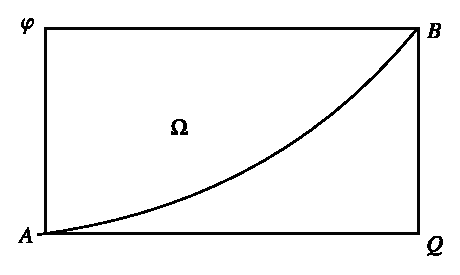
\includegraphics{6.eps}
\end{figure}
\begin{align*}
\int F \ dx \ dy &= \int \dfrac{\partial u}{\partial x \partial y}dx \ dy\\[3pt]
&= -\frac{1}{2}\int\limits^{P}_{B}\frac{\partial u}{\partial x} dx +\frac{1}{2}\int\limits^{A}_{P}\frac{\partial u}{\partial y}dy + \frac{1}{2}\int\limits^{B}_{A}\left(-\frac{\partial u}{\partial x}dx+\frac{\partial u}{\partial y}dy\right)\\[3pt]
&= \frac{1}{2}(u(B)-u(P)+\frac{1}{2}(u(A)-u(P))+\frac{1}{2}\int\limits^{B}_{A}-\frac{\partial u}{\partial x}dx+\frac{\partial u}{\partial y}dy.
\end{align*}
\footnote[7]{Hence 
$$
u(P)=-\int\limits_{\Omega} F \ dx \ dy +\frac{1}{2}(u(A)+u(B))+\frac{1}{2}\int\limits^{B}_{A}\frac{\partial u}{\partial x}dx-\frac{\partial u}{\partial y}dy
$$}

When $Q$ is below the curve, we have
$$
u(Q)=-\int\limits_{\Omega} F \ dx \ dy +\frac{1}{2}(u(A)+u(B))-\frac{1}{2}\int\limits^{B}_{A}\left(\frac{\partial u}{\partial x}dx-\frac{\partial u}{\partial y}\right)dy
$$

When the initial data are zero on $S$, we have in this case
$$
u(P)=-\int\limits_{\Omega}F \ dx \ dy.
$$

We will not check here that the function $u(P)$ defined by this formula effectively solves the Cauchy problem. This will be done in a more general context later.

\section*{Riemann's Formula:}\pageoriginale

We will now generalise the above representation of the solution of the Cauchy problem to the case $Lu=F$ where $L$ is an hyperbolic operator of the form:
$$
L=\frac{\partial^{2}}{\partial x\partial y}+a(x,y)\frac{\partial}{\partial x}+b(x,y)\frac{\partial}{\partial y}+c(x,y)
$$
where $a$, $b$, $c$ are smooth function (Essentially every hyperbolic operator in two variables is of this form at least locally. See the appendix).

We consider the adjoint operator $L^{\ast}$ given by
$$
L^{\ast}(v)=\frac{\partial^{2}v}{\partial x\partial y}-\frac{\partial}{\partial x}(av)-\frac{\partial}{\partial y}(bv)+cv.
$$
A simple calculation yields the formula
$$
vL(u)-uL^{\ast}(v)=\frac{\partial Q}{\partial x}-\frac{\partial P}{\partial y}
$$
where
\begin{align*}
P &= \frac{1}{2}\left(u\frac{\partial v}{\partial x}-v\frac{\partial u}{\partial x}\right)-b \ u \ v\\[3pt]
Q &= \frac{1}{2}\left(v\frac{\partial u}{\partial y}-u\frac{\partial v}{\partial y}\right)+a \ u \ v,
\end{align*}
so that we have for a bounded open set $\Omega$ with piecewise smooth boundary.
$$
\int\limits_{\Omega}vL(u)-uL^{\ast}(v)=\int\limits_{\partial \Omega}Pdx+Qdy
$$
We now apply this to the domain $\Omega$ in the previous section.
\begin{figure}[H]
\centering
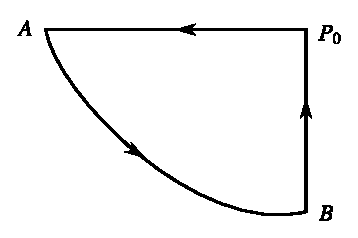
\includegraphics{7.eps}
\end{figure}

We have
%page 12


